\chapter{Escolha dos Sensores}\label{cap:sensores}
% Revisão de estudos sobre precisão, limitações e condições ambientais que afetam os sensores

%     Precisão dos sensores em diferentes condições ambientais (chuva, neblina, iluminação, etc.).

%     Limitações de cada tecnologia: reflexões, interferências e variações de leitura.

%     Comparação entre sensores e suas aplicações em diferentes cenários.
% - Sensores Ultrassônicos  
%   - Interferência em superfícies irregulares  
%   - Sensibilidade a temperatura e umidade  
%   - Melhor para curtas distâncias  
% - Sensores LiDAR  
%   - Alta precisão e longo alcance  
%   - Interferência em névoa e chuva  
%   - Custo mais elevado  
% - Câmeras com IA  
%   - Depende da iluminação do ambiente  
%   - Requer processamento computacional  
%   - Pode ser treinado para diferentes cenários  

\section{Sensores utilizados}
Os sensores utilizados neste trabalho foram selecionados com base em suas características técnicas, custo e aplicabilidade no monitoramento do nível de rios. Os sensores analisados são:
\begin{itemize}
    \item \textbf{Sensores LiDAR:} TF-Luna, TF-Nova.
    \item \textbf{Sensores Ultrassônicos:} JSN SR04T, HC-SR04.
    \item \textbf{Sensor com Câmera e IA:} ESP-CAM com modelo de inteligência artificial para medição de nível d'água.
\end{itemize}
Neste capítulo, serão apresentados os três tipos de sensores que foram analisados neste trabalho. A escolha dos sensores foi baseada em suas características técnicas, custo e aplicabilidade no monitoramento do nível de rios. Os sensores selecionados são: sensores ultrassônicos, sensores LiDAR e câmeras. A seguir, serão descritas as principais características de cada um deles.

% Definição dos sensores que serão testados (marcas, modelos e especificações técnicas)

% Descrição detalhada de cada sensor, incluindo:

% 	Tecnologia utilizada.

% 	Alcance mínimo e máximo.

% 	Precisão e taxa de atualização.

% 	Influência de fatores ambientais.
\section{Sensores Ultrassônicos}
Os sensores ultrassônicos são dispositivos que utilizam ondas sonoras para medir distâncias. Eles emitem um pulso de som e medem o tempo que leva para o eco retornar ao sensor. Essa tecnologia é amplamente utilizada em aplicações de automação e robótica, devido à sua precisão e baixo custo.

\subsection{JSN SR04T}
O JSN SR04T é um sensor ultrassônico de alta precisão, projetado para medir distâncias em ambientes externos. Ele possui um alcance de até 4 metros e é resistente à água, o que o torna ideal para aplicações em ambientes úmidos. O sensor é fácil de instalar e pode ser integrado a microcontroladores como Arduino e Raspberry Pi.
Ficha técnica:
\begin{itemize}
	\item Alcance: 20 cm a 4 m
	\item Precisão: ±1 cm
	\item Tensão de operação: 5 V
	\item Consumo de corrente: 15 mA
	\item Temperatura de operação: -20 °C a +70 °C
	\item Umidade de operação: 0\% a 100\%
	\item Resistência à água: IP67
	\item Taxa de atualização: 10 Hz
	\item Dimensões: 45 mm x 20 mm x 15 mm
	\item Peso: 20 g
\end{itemize}

\subsection{HC-SR04}
O HC-SR04 é um sensor ultrassônico amplamente utilizado em projetos de robótica e automação. Ele possui um alcance de até 4 metros e é conhecido por sua precisão e baixo custo. O sensor é fácil de usar e pode ser conectado a microcontroladores como Arduino e Raspberry Pi. No entanto, o HC-SR04 não é resistente à água, o que limita sua aplicação em ambientes úmidos.
Ficha técnica:
\begin{itemize}
	\item Alcance: 2 cm a 4 m
	\item Precisão: ±3 mm
	\item Tensão de operação: 5 V
	\item Consumo de corrente: 15 mA
	\item Temperatura de operação: -15 °C a +70 °C
	\item Umidade de operação: 0\% a 90\%
	\item Resistência à água: Não
	\item Taxa de atualização: 40 Hz
	\item Dimensões: 45 mm x 20 mm x 15 mm
	\item Peso: 20 g
\end{itemize}
\section{Sensores LiDAR}
Os sensores LiDAR (Light Detection and Ranging) utilizam luz laser para medir distâncias. Eles emitem pulsos de luz e medem o tempo que leva para o eco retornar ao sensor. Essa tecnologia é amplamente utilizada em aplicações de mapeamento e monitoramento ambiental, devido à sua alta precisão e capacidade de gerar dados tridimensionais.
Ficha técnica:
\begin{itemize}
	\item Alcance: 0,1 m a 12 m
	\item Precisão: ±1 cm
	\item Tensão de operação: 5 V
	\item Consumo de corrente: 100 mA
	\item Temperatura de operação: -10 °C a +50 °C
	\item Umidade de operação: 0\% a 95\%
	\item Resistência à água: Não
	\item Taxa de atualização: 100 Hz
	\item Dimensões: 45 mm x 20 mm x 15 mm
	\item Peso: 20 g
	\item Tecnologia: Laser de pulso
	\item Tipo de saída: Serial TTL
	\item Protocolo: UART
	\item Interface: UART
	\item Ângulo de visão: 270°
	\item Resolução: 1 cm
	\item Precisão: ±1 cm
	\item Taxa de amostragem: 100 Hz
	\item Distância mínima: 0,1 m
	\item Distância máxima: 12 m
	\item Temperatura de operação: -10 °C a +50 °C
	\item Umidade de operação: 0\% a 95\%
	\item Resistência à água: Não	
	\item Dimensões: 45 mm x 20 mm x 15 mm
	\item Peso: 20 g
\end{itemize}
\subsection{TF-Luna}
O TF-Luna é um sensor LiDAR de baixo custo, projetado para aplicações de medição de distância. Ele possui um alcance de até 8 metros e é conhecido por sua precisão e facilidade de uso. O sensor pode ser integrado a microcontroladores como Arduino e Raspberry Pi, tornando-o uma opção popular para projetos de robótica e automação.
Ficha técnica:
\begin{itemize}
	\item Alcance: 0,2 m a 8 m
	\item Precisão: ±1 cm
	\item Tensão de operação: 5 V
	\item Consumo de corrente: 100 mA
	\item Temperatura de operação: -10 °C a +50 °C
	\item Umidade de operação: 0\% a 95\%
	\item Resistência à água: Não
	\item Taxa de atualização: 100 Hz
	\item Dimensões: 45 mm x 20 mm x 15 mm
	\item Peso: 20 g
	\item Tecnologia: Laser de pulso
	\item Tipo de saída: Serial TTL
	\item Protocolo: UART
	\item Interface: UART
	\item Ângulo de visão: 270°
	\item Resolução: 1 cm
	\item Precisão: ±1 cm
	\item Taxa de amostragem: 100 Hz
	\item Distância mínima: 0,2 m
	\item Distância máxima: 8 m
	\item Temperatura de operação: -10 °C a +50 °C
	\item Umidade de operação: 0\% a 95\%
	\item Resistência à água: Não	
	\item Dimensões: 45 mm x 20 mm x 15 mm
	\item Peso: 20 g
	\item Tipo de saída: Serial TTL
\end{itemize}
\begin{figure}[h]
	\begin{lstlisting}[caption={Exemplo de um schema no Prisma.}, label={code:prisma}]
	generator client {
		provider = "prisma-client-js"
	}
	
	datasource db {
		provider = "postgresql"
		url      = env("DATABASE_URL")
	}
	
	model User {
		id        String        @id @unique @default(uuid())
		email     String        
		password  String
		cpf_cnpj  String        @unique
		name      String
		role      RoleEnumType? @default(user)
		createdAt DateTime      @default(now())
		updatedAt DateTime      @updatedAt
	}
	
	enum RoleEnumType {
		user
		admin
	}
		
	\end{lstlisting}
	
	\fonte{Criado pelo autor.}
	\end{figure}
\subsection{TF-Nova}
O TF-Nova é um sensor LiDAR de alta precisão, projetado para aplicações de mapeamento e monitoramento ambiental. Ele possui um alcance de até 12 metros e é conhecido por sua capacidade de gerar dados tridimensionais. O sensor pode ser integrado a microcontroladores como Arduino e Raspberry Pi, tornando-o uma opção popular para projetos de robótica e automação.
Ficha técnica:
\begin{itemize}
	\item Alcance: 0,1 m a 12 m
	\item Precisão: ±1 cm
	\item Tensão de operação: 5 V
	\item Consumo de corrente: 100 mA
	\item Temperatura de operação: -10 °C a +50 °C
	\item Umidade de operação: 0\% a 95\%
	\item Resistência à água: Não
	\item Taxa de atualização: 100 Hz
	\item Dimensões: 45 mm x 20 mm x 15 mm
	\item Peso: 20 g
	\item Tecnologia: Laser de pulso
	\item Tipo de saída: Serial TTL
	\item Protocolo: UART
	\item Interface: UART
	\item Ângulo de visão: 270°
	\item Resolução: 1 cm
	\item Precisão: ±1 cm
	\item Taxa de amostragem: 100 Hz
	\item Distância mínima: 0,1 m
	\item Distância máxima: 12 m
	\item Temperatura de operação: -10 °C a +50 °C
	\item Umidade de operação: 0\% a 95\%
	\item Resistência à água: Não	
	\item Dimensões: 45 mm x 20 mm x 15 mm
	\item Peso: 20 g
	\item Tipo de saída: Serial TTL
\end{itemize}

\begin{figure}[h]
	\centering
	\caption{Arquitetura do Sistema.}
	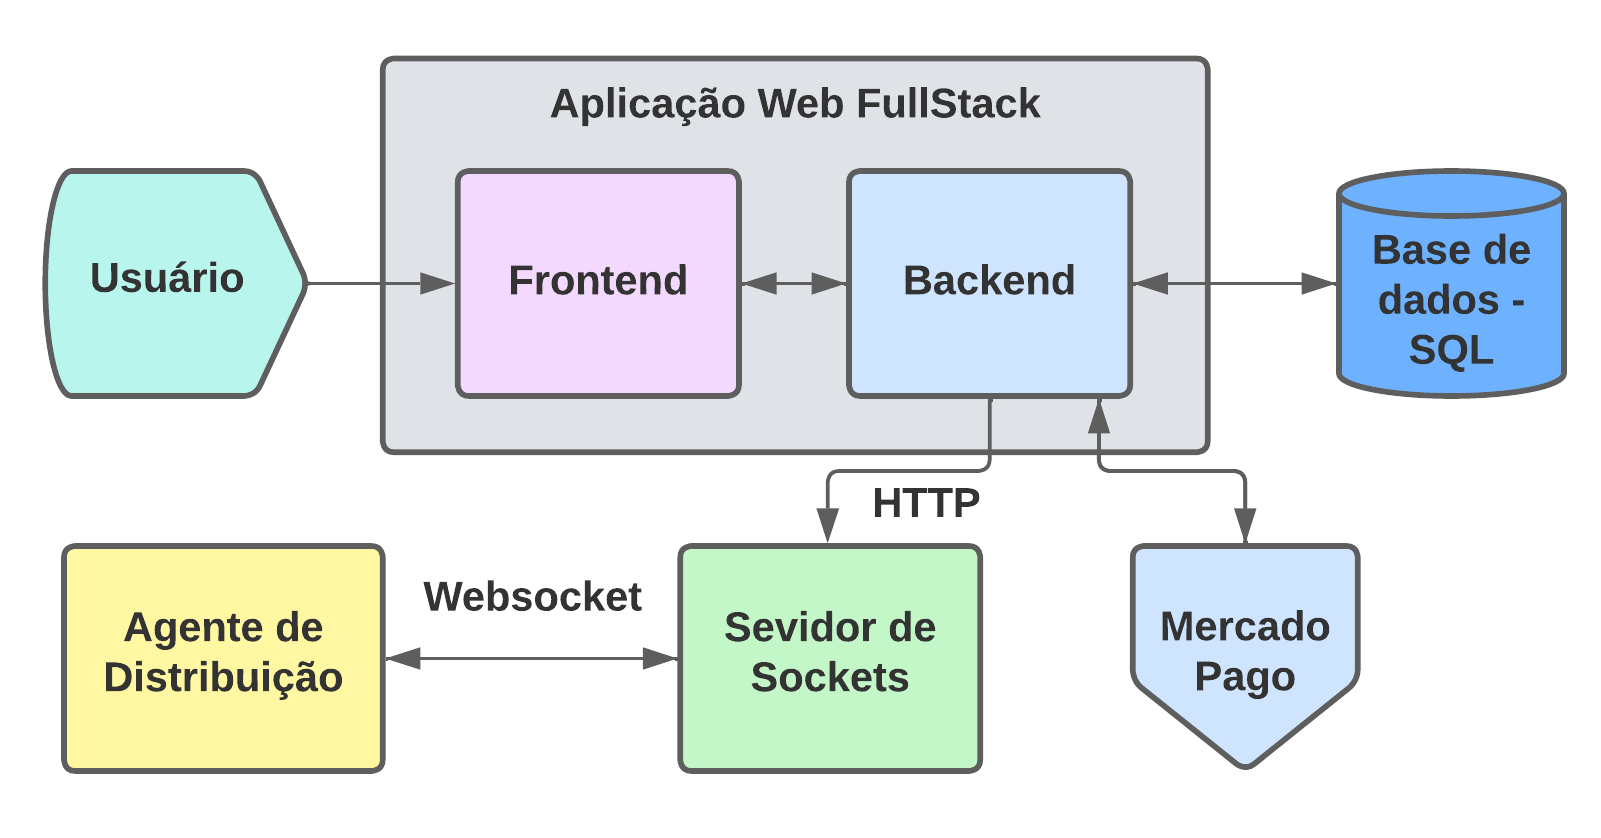
\includegraphics[width=1\textwidth]{figuras/Arquitetura.png}
	\fonte{Criado pelo autor.}
	\label{fig:system_architecture}
\end{figure}

\section{Câmeras}
As câmeras são dispositivos que capturam imagens e vídeos. Elas podem ser utilizadas em diversas aplicações, incluindo monitoramento ambiental e reconhecimento de padrões. As câmeras modernas são equipadas com tecnologia de inteligência artificial, permitindo a análise de imagens em tempo real.
\subsection{ESP-CAM}
A ESP-CAM é uma câmera de baixo custo, projetada para aplicações de monitoramento e reconhecimento de padrões. Ela possui um módulo Wi-Fi integrado, permitindo a transmissão de imagens em tempo real. A câmera pode ser programada para realizar tarefas específicas, como detecção de movimento e reconhecimento facial, utilizando modelos de inteligência artificial.
A ESP-CAM é uma opção popular para projetos de automação e monitoramento ambiental, devido ao seu baixo custo e facilidade de uso. Ela pode ser integrada a microcontroladores como Arduino e Raspberry Pi, tornando-a uma opção versátil para diversas aplicações.
Ficha técnica:
\begin{itemize}
	\item Resolução: 640 x 480 pixels
	\item Tensão de operação: 5 V
	\item Consumo de corrente: 200 mA
	\item Temperatura de operação: -20 °C a +70 °C
	\item Umidade de operação: 0\% a 100\%
	\item Resistência à água: Não
	\item Taxa de atualização: 30 fps
	\item Dimensões: 45 mm x 20 mm x 15 mm
	\item Peso: 20 g
	\item Tecnologia: Câmera com IA
	\item Tipo de saída: Serial TTL
	\item Protocolo: UART
	\item Interface: UART
	\item Ângulo de visão: 90°
	\item Resolução: 640 x 480 pixels
	\item Precisão: ±1 cm
	\item Taxa de amostragem: 30 fps
	\item Distância mínima: 0,1 m
	\item Distância máxima: 12 m
	\item Temperatura de operação: -20 °C a +70 °C
	\item Umidade de operação: 0\% a 100\%
	\item Resistência à água: Não	
	\item Dimensões: 45 mm x 20 mm x 15 mm
	\item Peso: 20 g
	\item Tipo de saída: Serial TTL
\end{itemize}

\begin{table}[htb]
	\ABNTEXfontereduzida
	\caption{\label{tab:Tab_1}Preços dos planos de hospedagem em nuvem.}
 \begin{center}
	\begin{tabular}{@{}p{2.0cm}p{1.5cm}p{3.0cm}p{3.5cm}@{}}
		\toprule
		\textbf{Plataforma} & \textbf{Plano} & \textbf{Preço} & \textbf{Limites} \\ \midrule
		Vercel & Hobby & \ Gratuito & Projetos pessoais ou não comerciais. Deploy a partir do CLI ou integrações git. HTTPS/SSL automático. \\
		Vercel & Pro & \$20 por membro da equipe por mês. & 1TB de banda. 1000 GB/horas de execução. \\
		Vercel & Enterprise & Personalizado. & Infraestrutura de build isolada, em hardware melhor, sem filas. \\
		Railway & Starter & Gratuito & \$5.00 em créditos de recursos todos os meses com tempo de execução de 500 horas. \\
		Railway & Hobby & \$10 em créditos por mês & 8 GB de RAM / 8 vCPU por serviço \\
		Railway & Pro & \$20 por mês & Acesso compartilhado ao espaço de trabalho para equipes. \\
		Railway & Enterprise & Personalizado & Personalizado \\
		ElephantSQL & Tiny & Gratuito & 20 MB, 5 conexões concorrentes \\
		ElephantSQL & Simple & \$5 por mês & 500 MB, 10 conexões concorrentes \\
            ElephantSQL & Enormous & \$199 por mês & 250 GB, centenas de conexões concorrentes \\
  \bottomrule
	\end{tabular}
 \end{center}
	\fonte{Sites das respectivas plataformas.}
\end{table}

% Tabela comparativa entre os sensores

\begin{table}
	\ABNTEXfontereduzida
	\caption{\label{tab:Tab_2}Tabela comparativa entre os sensores.}
 \begin{center}
	\begin{tabular}{@{}p{2.0cm}p{1.5cm}p{3.0cm}p{3.5cm}@{}}
		\toprule
		\textbf{Sensor} & \textbf{Tipo} & \textbf{Alcance} & \textbf{Precisão} \\ \midrule
		JNS SR04T & Ultrassônico & 20 cm a 4 m & ±1 cm \\
		HC-SR04 & Ultrassônico & 2 cm a 4 m & ±3 mm \\
		TF-Luna & LiDAR & 0,2 m a 8 m & ±1 cm \\
		TF-Nova & LiDAR & 0,1 m a 12 m & ±1 cm \\
		ESP-CAM & Câmera com IA & 0,1 m a 12 m & ±1 cm \\ 
  \bottomrule
	\end{tabular}
 \end{center}
	\fonte{Criado pelo autor.}
	\label{tab:comparativo}
\end{table}


\chapter{Metodologia experimental}\label{cap:metodologia}
% Ambiente de testes: Escolha de locais representativos, como trechos de rios na região de Itajaí e Vale.

% Procedimento de testes:

% Instalar os sensores em diferentes condições (alturas, distâncias e superfícies).

% Medir a variação das leituras em diferentes condições climáticas.

% Comparar resultados entre sensores para verificar a confiabilidade.

% Métricas de avaliação:

% Precisão da medição em comparação com referência manual.

% Estabilidade da leitura em diferentes condições ambientais.

% Tempo de resposta dos sensores.
% Estruturação da metodologia experimental

% Ambiente de testes: Escolha de locais representativos, como trechos de rios na região de Itajaí e Vale.

% Procedimento de testes:

% 	Instalar os sensores em diferentes condições (alturas, distâncias e superfícies).

% 	Medir a variação das leituras em diferentes condições climáticas.

% 	Comparar resultados entre sensores para verificar a confiabilidade.

% Métricas de avaliação:

% 	Precisão da medição em comparação com referência manual.

% 	Estabilidade da leitura em diferentes condições ambientais.

% % 	Tempo de resposta dos sensores.
% 1. Seleção dos sensores  
% 2. Definição do local de testes  
% 3. Instalação dos sensores  
% 4. Coleta de dados em diferentes condições  
% 5. Comparação dos resultados  
% 6. Análise da viabilidade de cada sensor  

% Precisao e acuracia dos sensores

\section{Metodologia Experimental}
O estudo será conduzido em duas etapas principais: \textbf{testes em ambiente controlado} e \textbf{testes em condições reais}. O objetivo é comparar a precisão e acurácia dos sensores, verificar se suas especificações técnicas estão corretas e analisar seu desempenho em diferentes condições ambientais.

\subsection{Testes em Ambiente Controlado}
Nesta etapa, os sensores serão avaliados em um ambiente estável e previsível, com iluminação adequada e sem interferências externas.

\subsubsection{Procedimentos}
\begin{enumerate}
    \item \textbf{Configuração e Calibração}
    \begin{itemize}
        \item Instalar cada sensor em um suporte fixo a uma altura conhecida.
        \item Calibrar os sensores conforme as especificações do fabricante.
        \item Definir uma referência de medição utilizando instrumentos de alta precisão.
    \end{itemize}
    \item \textbf{Teste de Precisão e Acurácia}
    \begin{itemize}
        \item Medir distâncias conhecidas e comparar com os valores obtidos.
        \item Repetir medições múltiplas vezes e calcular média e desvio padrão.
        \item Determinar a acurácia comparando com a referência.
    \end{itemize}
    \item \textbf{Teste de Limite de Alcance}
    \begin{itemize}
        \item Posicionar alvos em diferentes distâncias dentro do alcance especificado.
        \item Verificar até que ponto cada sensor fornece medições estáveis.
    \end{itemize}
    \item \textbf{Teste de Sensibilidade a Condições Variáveis}
    \begin{itemize}
        \item Testar os sensores com diferentes superfícies de medição (água limpa, água com impurezas, materiais reflexivos, etc.).
        \item Alterar a inclinação do sensor para verificar variações nas leituras.
    \end{itemize}
\end{enumerate}

\subsection{Testes em Condições Reais}
Os sensores serão instalados em corpos d’água reais para avaliar seu desempenho em longo prazo, considerando fatores ambientais como variações climáticas e interferências externas.

\subsubsection{Procedimentos}
\begin{enumerate}
    \item \textbf{Instalação dos Sensores}
    \begin{itemize}
        \item Fixar os sensores em estruturas adequadas na margem ou sobre a superfície da água.
        \item Garantir posicionamento adequado para evitar interferências externas.
    \end{itemize}
    \item \textbf{Coleta de Dados em Diferentes Condições}
    \begin{itemize}
        \item Realizar medições em diferentes horários do dia.
        \item Comparar medições em diferentes condições climáticas.
        \item Monitorar a estabilidade das leituras ao longo do tempo.
    \end{itemize}
    \item \textbf{Validação com Medições de Referência}
    \begin{itemize}
        \item Utilizar uma régua linimétrica ou outro método manual para comparação.
        \item Analisar variações e discrepâncias entre os sensores.
    \end{itemize}
    \item \textbf{Análise da Durabilidade e Confiabilidade}
    \begin{itemize}
        \item Avaliar possíveis degradações no desempenho devido a sujeira, umidade ou variações ambientais.
        \item Medir o consumo de energia ao longo do tempo.
    \end{itemize}
\end{enumerate}

\section{Métricas de Avaliação}
Os sensores serão comparados com base nos seguintes critérios:
\begin{itemize}
    \item \textbf{Precisão:} Variação das medições em relação ao valor real.
    \item \textbf{Acurácia:} Diferença entre o valor medido e a referência.
    \item \textbf{Estabilidade:} Consistência das medições ao longo do tempo.
    \item \textbf{Interferência Ambiental:} Impacto de fatores externos como iluminação, vento e temperatura.
    \item \textbf{Limite de Alcance:} Distância máxima em que o sensor fornece leituras confiáveis.
    \item \textbf{Confiabilidade:} Desempenho após longo período de operação.
\end{itemize}

\section{Fluxograma da Metodologia}

\begin{itemize}
    \item \textbf{Testes em Ambiente Controlado}
    \begin{itemize}
        \item Configuração e calibração
        \item Teste de precisão e acurácia
        \item Teste de limite de alcance
        \item Teste com diferentes superfícies
    \end{itemize}
    \item \textbf{Testes em Condições Reais}
    \begin{itemize}
        \item Instalação dos sensores em corpos d'água
        \item Coleta de dados em diferentes condições ambientais
        \item Comparação com medições de referência
        \item Análise da durabilidade e confiabilidade
    \end{itemize}
    \item \textbf{Análise e Comparação dos Resultados}
    \begin{itemize}
        \item Comparação entre sensores
        \item Identificação de limitações e recomendações
        \item Conclusões sobre a melhor tecnologia para monitoramento
    \end{itemize}
\end{itemize}


\chapter{Arquitetura do sistema}\label{cap:arquitetura}


\chapter{Implementação}\label{cap:desenvolvimento}

\chapter{Resultados}\label{cap:resultados}

\section{Hospedagem e custos}\label{cap:host}

\section{Considerações finais} \label{cap:final}


